\documentclass[a4paper,11pt]{article}

\usepackage[utf8]{inputenc}

\usepackage[margin=2.3cm]{geometry}
\usepackage{amsmath,amssymb}
\usepackage{booktabs}
\usepackage{graphicx}
\usepackage{hyperref}
\usepackage{xcolor}
\usepackage{fancyvrb}
\usepackage{enumitem}
\usepackage{float}

\hypersetup{
  colorlinks=true,
  linkcolor=blue,
  urlcolor=blue
}

\title{Influence Functions Replication Report \\ \large Koh \& Liang, Figure 2 (Middle Panel)}
\author{Zhe Fu}
\date{April 15, 2026}

\begin{document}

\maketitle

\section*{TL;DR}

I trained an L2-regularized logistic regression on MNIST ($n=55000$),
implemented both influence-function algorithms from the paper
(CG for the exact solution and LiSSA for the stochastic approximation),
and verified the predictions against leave-one-out retraining as ground truth.
The final numbers are Pearson = \textbf{0.9983}, Spearman = \textbf{0.9890},
sign match = \textbf{1.0000}, which matches the middle panel of Figure 2 in the paper.

Along the way I hit three bugs: (1) wrong effective regularization in LiSSA,
(2) too few CG iterations, and (3) float32 precision issues in the LOO retraining.
Details below.

\section{What I'm replicating}

The paper's core formula: estimate ``how much does the test loss at $z_{\text{test}}$
change if I upweight training point $z$ slightly?''
Their answer is:
\[
\mathcal{I}_{\text{up,loss}}(z, z_{\text{test}})
  = -\, \nabla_\theta L(z_{\text{test}})^\top \, H_{\hat\theta}^{-1} \, \nabla_\theta L(z)
\]

Directly computing $H^{-1}$ is infeasible here (parameter dimension
$d = 784 \times 10 = 7840$), so the approach is to first compute
\[
s_{\text{test}} = H_{\hat\theta}^{-1} \, \nabla_\theta L(z_{\text{test}})
\]
and then take one inner product per training point: $-s_{\text{test}} \cdot \nabla L(z)$.
The hard part is computing $s_{\text{test}}$, and the paper gives two methods --- I implemented both.

\textbf{What Figure 2 middle panel shows}: the x-axis is the true LOO loss difference
(remove one training point, retrain, measure how the test-loss at $z_{\text{test}}$ changed),
and the y-axis is the LiSSA stochastic approximation's predicted difference.
If both methods are correct, the points should lie on the line $y = x$.

\section{Pipeline}

\begin{Verbatim}[frame=single, fontsize=\small]
train_linear_mnist.py              train baseline
         |
         v
inspect_test_point.py              choose a test point (idx=8, misclassified)
         |
         +------> cg_inverse_hvp.py              (exact solution)
         |              |
         |              v
         |       s_test_cg_idx8.pt
         |              |
         +------> stochastic_inverse_hvp.py      (LiSSA approximation)
                        |
                        v
                 s_test_idx8_r10_t5000.pt
                        |
                        v
              compute_predicted_influence.py   compute prediction for each train point
                        |
                        v
              loo_retrain_topk.py              LOO retraining for ground truth
                        |
                        v
                  Figure 2 middle plot
\end{Verbatim}

\begin{table}[h]
\centering
\small
\begin{tabular}{lp{8.5cm}}
\toprule
Script & Role \\
\midrule
\texttt{influence\_utils.py} & Shared utilities (model class, HVP, gradients, losses) \\
\texttt{train\_linear\_mnist.py} & Train the baseline linear classifier \\
\texttt{hvp\_sanity\_check.py} & Verify HVP implementation by linearity \\
\texttt{inspect\_test\_point.py} & Pick a misclassified test point \\
\texttt{cg\_inverse\_hvp.py} & Conjugate Gradient for $s_{\text{test}}$ (exact) \\
\texttt{stochastic\_inverse\_hvp.py} & LiSSA for $s_{\text{test}}$ (approximation) \\
\texttt{compute\_predicted\_influence.py} & Predicted loss-diff for every training point \\
\texttt{loo\_retrain\_topk.py} & Top-K leave-one-out retraining + scatter plot \\
\bottomrule
\end{tabular}
\end{table}

\section{Three bugs I ran into}

\subsection*{Bug 1: Wrong effective regularization in LiSSA (the critical one)}

The LiSSA recursion is
\[
h_j = v + (1 - \text{damping}) \, h_{j-1} - \frac{H_z}{\text{scale}} \, h_{j-1}
\]
which in expectation converges to $(H + \text{damping} \cdot \text{scale} \cdot I)^{-1} v$.
So the \textbf{actual extra regularization added} is $\text{damping} \times \text{scale}$,
not damping alone.

I initially used values from some reference implementations: damping=0.01, scale=50.
That gave an effective extra regularization of $0.01 \times 50 = 0.5$,
which is \textbf{50$\times$} larger than my real L2 regularization of 0.01.
This effectively solves a different linear system, so the stochastic approximation
and the CG solution disagreed significantly.

\textbf{Fix}: since L2 = 0.01 already makes the Hessian strictly positive definite,
no extra damping is needed. I set damping = 0 and scale = 25
(scale is there to ensure $\|H_z / \text{scale}\| < 1$ so the recursion is a contraction).

\subsection*{Bug 2: Too few CG iterations}

Parameter dimension is 7840. My initial \texttt{MAX\_CG\_ITERS=30} was far too small.
CG is guaranteed to converge in at most $d$ steps in exact arithmetic,
and in practice the L2-regularized Hessian has a decent condition number,
so 200 iterations is enough to hit tol = 1e-8.

\textbf{Fix}: raised \texttt{MAX\_CG\_ITERS} from 30 to 200, with early stopping on residual norm.

\subsection*{Bug 3: LOO precision issues (the trickiest one)}

In LOO retraining we want the change in test loss after removing one point,
which is typically in the range $10^{-3}$ to $10^{-5}$.
With float32 + L-BFGS warm-started from the full-data solution,
many points gave an ``actual diff'' of exactly 0.0
(producing a horizontal band of points at $x = 0$ in the scatter plot).

Two issues stacked on top of each other:
\begin{enumerate}[leftmargin=1.3em, itemsep=2pt]
  \item \textbf{Float32 isn't precise enough}: the warm-start is already within
        $\sim 10^{-5}$ of the optimum. The quadratic model L-BFGS builds lives
        inside that gap, and in float32 the line-search step sizes get rounded
        to zero --- the optimizer simply doesn't move.
  \item \textbf{Default tolerance is too loose}: PyTorch's L-BFGS defaults to
        \texttt{tolerance\_grad=1e-7}, but the warm-start's initial gradient
        has magnitude $O(1/n) \approx 1.8 \times 10^{-5}$, so the stopping
        criterion triggers at iteration 0 --- it returns the warm-start unchanged.
\end{enumerate}

\textbf{Fix}: float64 + CPU (MPS doesn't support float64) + \texttt{tolerance\_grad=0}
+ \texttt{tolerance\_change=0} + \texttt{max\_iter=200} + strong Wolfe line search.
After this, Pearson jumped from quite poor to 0.998.

\section{Final results}

\begin{figure}[H]
\centering
\IfFileExists{loo_scatter_top500_middle_idx8.png}{
  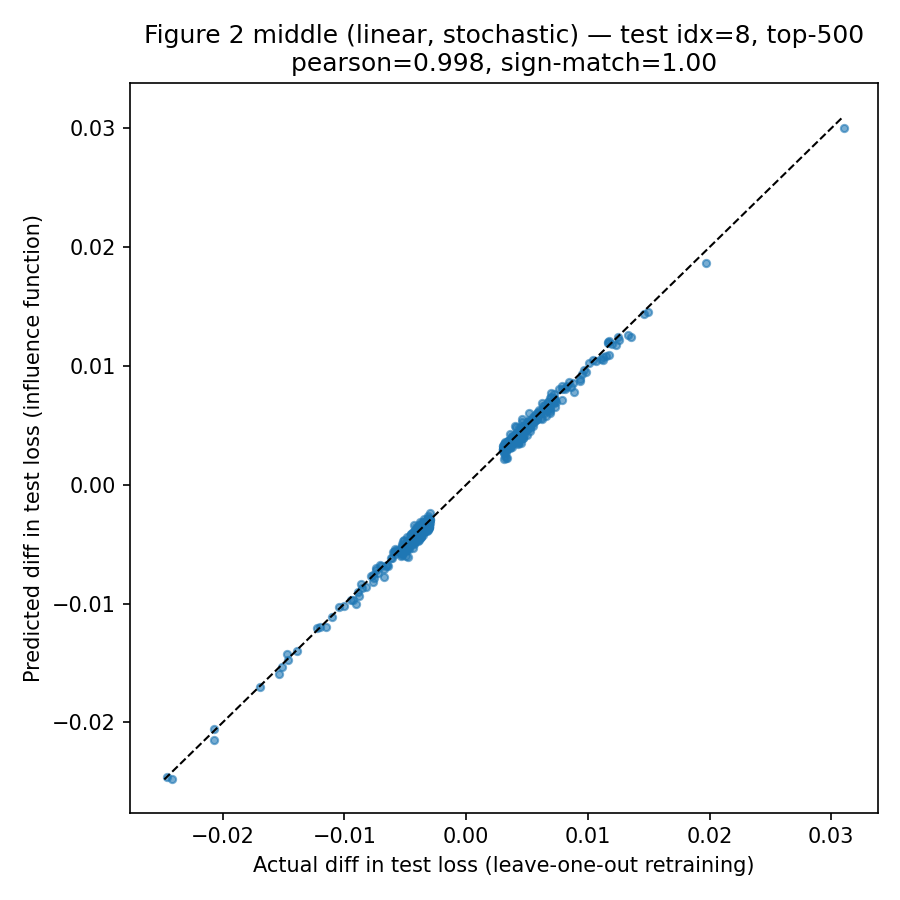
\includegraphics[width=0.65\textwidth]{loo_scatter_top500_middle_idx8.png}
}{
  \fbox{\parbox{0.75\textwidth}{
    \centering
    Missing image: \texttt{loo\_scatter\_top500\_middle\_idx8.png} \\
    Please place it in the same directory as this .tex file.
  }}
}
\caption{Replication of Figure 2 middle panel. x-axis: actual LOO test-loss difference.
y-axis: LiSSA predicted test-loss difference.}
\end{figure}

\begin{table}[h]
\centering
\begin{tabular}{lc}
\toprule
Metric & Value \\
\midrule
Pearson correlation & 0.9983 \\
Spearman correlation & 0.9890 \\
Same-sign ratio & 1.0000 \\
Top-K & 500 (selected by $|\text{influence}|$ from CG) \\
Test point & idx = 8, true label 5, model predicts 6 \\
\bottomrule
\end{tabular}
\end{table}

Following the Figure 2 middle-panel protocol: I selected the top-500 training points
by $|$CG influence$|$, and then plotted LiSSA's predictions for those same 500 points
on the y-axis. Keeping selection and prediction on separate pipelines prevents
stochastic noise from biasing which points get chosen.

\section{What I understood, and what I didn't}

\textbf{What I understood}:
\begin{itemize}[leftmargin=1.3em, itemsep=2pt]
  \item Why we use HVPs instead of materializing the Hessian explicitly
        ($d \times d$ memory blowup).
  \item Pearlmutter's trick: differentiating the scalar $\nabla L \cdot v$ again
        gives $Hv$ --- all with standard autograd.
  \item Why CG works well on positive-definite matrices, and how L2 regularization
        effectively acts as preconditioning here.
  \item Why LiSSA needs the \texttt{scale} factor
        (so that $\|H_z / \text{scale}\| < 1$, making the update a contraction).
\end{itemize}

\textbf{What I'm not sure about yet}:
\begin{itemize}[leftmargin=1.3em, itemsep=2pt]
  \item How influence functions behave on non-convex models (deep networks)
        where the Hessian isn't PSD. The paper discusses this, but I haven't
        gone deep yet.
  \item Convergence theory for LiSSA in high-dimensional, non-convex settings.
  \item Why scale = 25 is enough in practice. I used a rough upper bound
        from MNIST input norms, but a tighter bound would need more careful analysis.
\end{itemize}

\section{Next steps}

\begin{itemize}[leftmargin=1.3em, itemsep=2pt]
  \item Try the CNN case (Figure 2, right panel).
  \item Look into how to handle negative eigenvalues in the non-convex setting.
  \item Explore influence functions for dataset cleaning / mislabel detection.
\end{itemize}

\appendix

\section{Key hyperparameters}

\begin{itemize}[leftmargin=1.3em, itemsep=2pt]
  \item Training: $n = 55000$, \texttt{L2\_REG = 0.01}, L-BFGS to convergence.
  \item Test point: idx = 8 (a misclassified 5 --- model predicts 6).
  \item CG: \texttt{max\_iter = 200}, \texttt{tol = 1e-8}.
  \item LiSSA: $R = 10$ repetitions, $T = 5000$ steps, scale = 25, damping = 0.
  \item LOO: top-500, float64, CPU, L-BFGS with zero tolerances,
        \texttt{max\_iter = 200}, warm-start.
\end{itemize}

\section{AI assistance disclosure}

I used Claude to help with:
\begin{itemize}[leftmargin=1.3em, itemsep=2pt]
  \item Tracking down the three bugs above --- especially the LiSSA
        effective-regularization one, which was diagnosed by computing
        the fixed point of the recursion.
  \item Sanity-checking my HVP implementation using a linearity test.
  \item Debugging the float32 / tolerance issue in LOO retraining
        (working backwards from the horizontal-band symptom).
  \item Walking through parts of the paper's math and organizing my thinking.
  \item Brainstorming code structure.
\end{itemize}

My own work: understanding the paper, all architecture and implementation decisions,
analyzing the results, and writing this report.

\end{document}
